\documentclass[10pt,aspectratio=169]{beamer}

\usetheme[progressbar=frametitle]{metropolis}
\usefonttheme{professionalfonts} 

\usepackage{appendixnumberbeamer}
\usepackage{amsmath}
\usepackage{bbm}
\usepackage[style=apa]{biblatex}
\addbibresource{bib/20241028.bib}

\usepackage{booktabs}
\newcommand{\tabitem}{~~\llap{\textbullet}~~}
\usepackage[scale=2]{ccicons}

\usepackage{pgfplots}
\usepgfplotslibrary{dateplot}
\usepackage{tikz}
\usetikzlibrary{decorations.pathreplacing,calc,tikzmark}

\usepackage{animate}
\usepackage{hyperref}
\usepackage{fdsymbol}
\usepackage{multirow}
\usepackage{longtable}

\usepackage[export]{adjustbox}
\tikzset{ffgcaption/.style={%
    anchor=south east,font=\tiny,
    text=white,fill=black,
    fill opacity=.5,text opacity=1,inner sep=2pt,
    text height=1ex,text depth=.25ex}}

% \fullframegraphic 
% renders a single image fullscreen, with an optional credit/caption in the 
% lower right corner.
% Usage: \fullframegraphic[some optional caption]{path/to/image}
% It does not crop the image, but leads to white borders if image does not match
% the aspect ratio of the slide. See commands \fullframegraphicw and
% \fullframegraphich below for cropping alternatives.
\newcommand{\fullframegraphic}[2][]{%
\begin{frame}[plain]%
\begin{tikzpicture}[remember picture,overlay]%
\node[at=(current page.center)] {%
\includegraphics[height=\paperheight,width=\paperwidth,keepaspectratio]{#2}%
};%
\ifx\relax#1\relax\else%
\node[at=(current page.south east),ffgcaption] {#1};%
\fi%
\end{tikzpicture}%
\end{frame}%
}

% \fullframegraphicw: scles image to frame width, cropping excess height.
% use for images that are "taller" than the frame aspect ratio
\newcommand{\fullframegraphicw}[2][]{%
\begin{frame}[plain]%
\begin{tikzpicture}[remember picture,overlay]%
\node[at=(current page.center)] {%
\includegraphics[min height=\paperheight,max width=\paperwidth,keepaspectratio]{#2}%
};%
\ifx\relax#1\relax\else%
\node[at=(current page.south east),ffgcaption] {#1};%
\fi%
\end{tikzpicture}%
\end{frame}%
}

% \fullframegraphich: scales image to frame height, cropping excess width.
% use for images that are wider than the frame aspect ratio
\newcommand{\fullframegraphich}[2][]{%
\begin{frame}[plain]%
\begin{tikzpicture}[remember picture,overlay]%
\node[at=(current page.center)] {%
\includegraphics[max height=\paperheight,min width=\paperwidth,keepaspectratio]{#2}%
};%
\ifx\relax#1\relax\else%
\node[at=(current page.south east),ffgcaption] {#1};%
\fi%
\end{tikzpicture}%
\end{frame}%
}

% \fullframegraphics: more customisable version of fullframegraphic, allowing
% a third argument to insert additional tikz commands for custom overlays.
% use when tooltips or highlights are required on a large image
\newcommand{\fullframegraphics}[3][]{%
\begin{frame}[plain]%
\begin{tikzpicture}[remember picture,overlay]%
\node[at=(current page.center)] {%
\includegraphics[height=\paperheight,width=\paperwidth,keepaspectratio]{#2}%
};%
\ifx\relax#1\relax\else%
\node[at=(current page.south east),ffgcaption] {#1};%
\fi%
#3%
\end{tikzpicture}%
\end{frame}%
}

% Custom command that adds journal abbreviation to cite
\DeclareCiteCommand{\journalcite}
  {\usebibmacro{prenote}} 
  {\printnames{labelname} 
   \setunit{\addcomma\space}
   \printfield{shortjournal} 
   \setunit{\addspace} 
   \printfield{year}}
  {\multicitedelim} 
  {\usebibmacro{postnote}} 

% Custom command that adds journal abbreviation to textcite
\DeclareCiteCommand{\journaltextcite}
  {\usebibmacro{prenote}}
  {\printnames{labelname} 
   (\printfield{shortjournal} 
   \setunit{\addspace} 
   \printfield{year})} 
  {\multicitedelim} 
  {\usebibmacro{postnote}} 


\usepackage{xspace}
\newcommand{\themename}{\textbf{\textsc{metropolis}}\xspace}

\title{Physician Training and Treatment Decisions}
\author{Shirley Cai}
\date{October 31, 2024}
\institute{Department of Economics\\Emory University}
% \titlegraphic{\hfill\includegraphics[height=1.5cm]{logo.pdf}}

\usepackage{textpos}
\addtobeamertemplate{frametitle}{}{%
\begin{textblock*}{10mm}(.88\textwidth,-.8cm)
% \includegraphics[height=0.55cm]{EU_hz_rev.png}
\end{textblock*}}

\begin{document}

\maketitle

\begin{frame}{Physician agency problem}
    \metroset{block = fill}
    \textbf{Physician treatment decisions encapsulate a principal-agent problem.}
    
    \begin{figure}
        \centering
        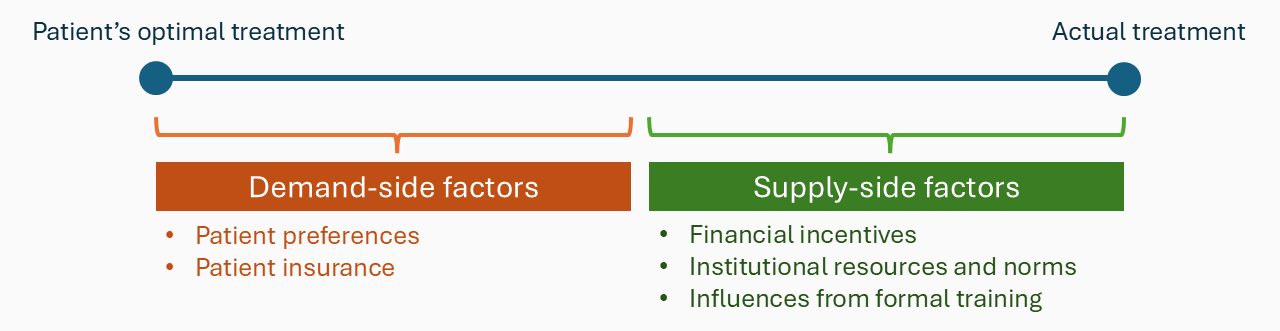
\includegraphics[width=1\linewidth]{image/gap-factors.png}
    \end{figure}

    $\to$ The actual treatment chosen may be very different from the patient's optimal treatment.
\end{frame}

\begin{frame}{Research question} \label{rq}
    \metroset{block = fill}
    What is the effect of treatment intensity a cardiologist is exposed to during medical school on their treatment intensity post-training?

    \vspace{5mm}
    \begin{block}{Treatment intensity}
        For a given year, 
            \begin{equation*}
                (\text{intensity}) = \frac{\text{number of invasive procedures}}{\text{number of unique patients}}.
            \end{equation*}
        \hyperlink{intensity}{\beamerbutton{Intensity specifics}}
    \end{block}
      
\end{frame}

\begin{frame}{Policy implications}
    Determining the importance of formal training among supply-side factors informs policy design. 
    \begin{figure}
        \centering
        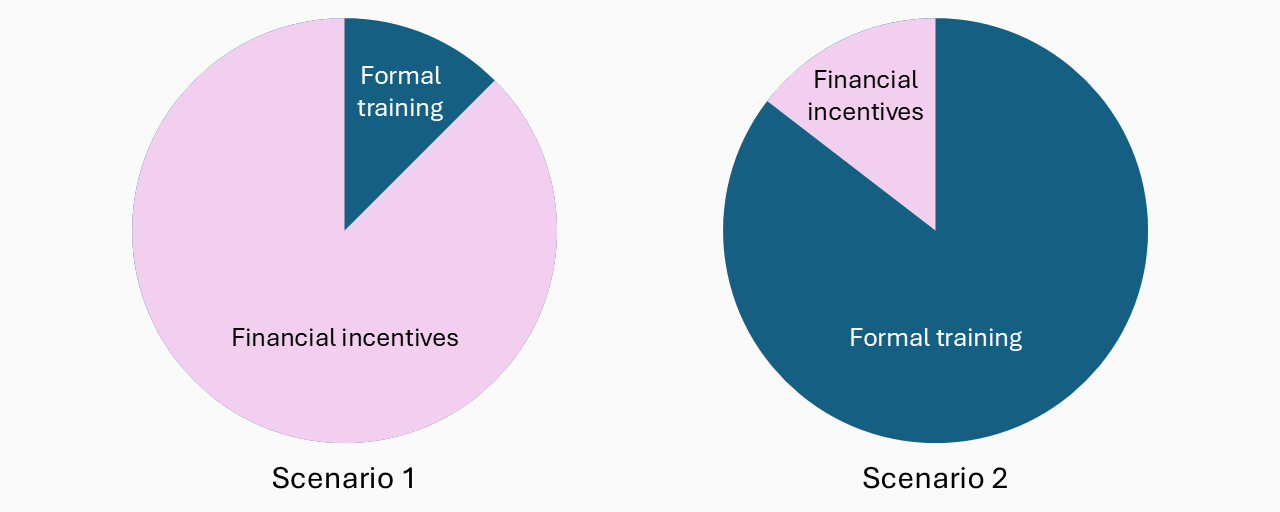
\includegraphics[width=\linewidth]{image/gap-supply-side.png}
    \end{figure}
\end{frame}

\begin{frame}{Cardiologist training pipeline}
    \begin{figure}
        \centering
        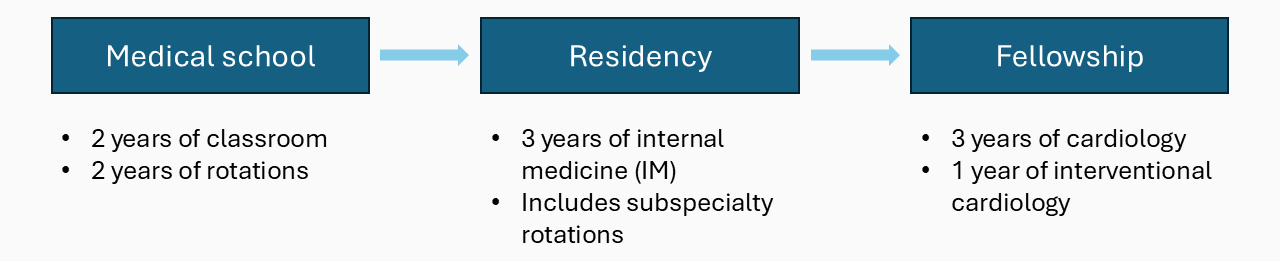
\includegraphics[width=\linewidth]{image/train-pipe.png}
    \end{figure}
\end{frame}

\begin{frame}{Geographic variation is evidence of difference practice styles}
    Different physician practice styles drive variation in healthcare utilization \tiny(\journalcite{cutler_physician_2019}, \journalcite{badinski_geographic_2023})\normalsize.
    \begin{figure}
        \centering
        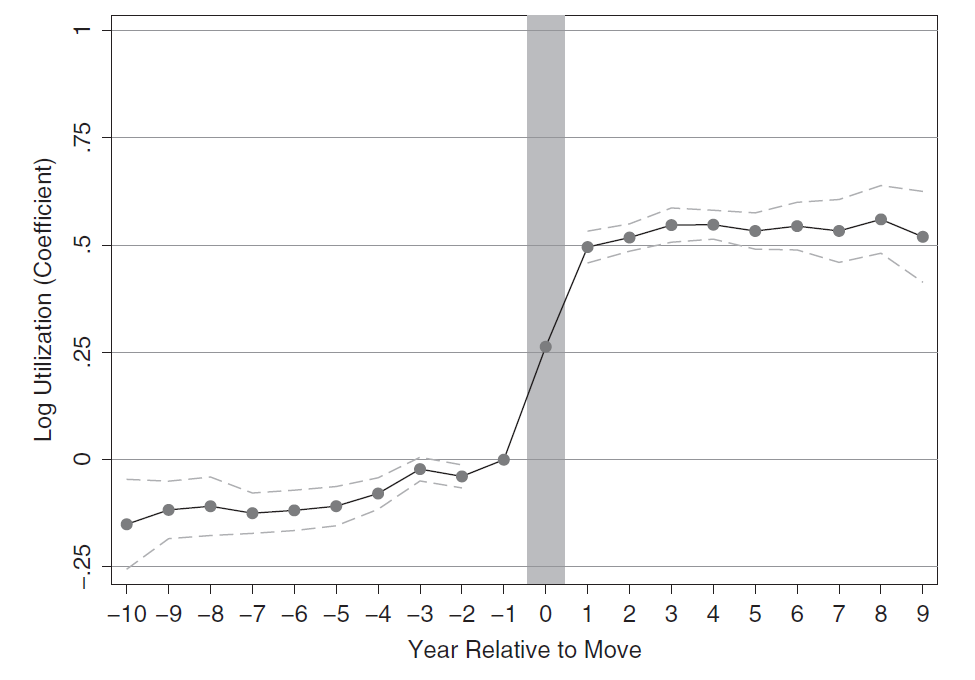
\includegraphics[width=0.55\linewidth]{image/finkelstein-fig6.png}
        \caption{Event study from \journaltextcite{finkelstein_sources_2016}}
    \end{figure}
\end{frame}

\begin{frame}{Previous literature}
    \metroset{block = fill}
    Different physician practice styles drive variation in healthcare utilization \tiny(\journalcite{cutler_physician_2019}, \journalcite{badinski_geographic_2023})\normalsize, but \textbf{it's unclear how these practice styles develop}.

    \vspace{2.5mm}
    \begin{block}{Formal training}
        \begin{itemize}
            \item Physicians from higher-ranked medical schools prescribe fewer opioids. \tiny(\journalcite{schnell_addressing_2018}) \normalsize
            \item Physicians from higher-ranked residency programs incur lower costs. \tiny(\journalcite{doyle_returns_2010}) \normalsize
            \item 2\% of variation in c-section rates is attributed to residency program. \tiny(\journalcite{epstein_formation_2009}) \normalsize 
        \end{itemize}
    \end{block}

    \vspace{2.5mm}
    \begin{block}{Practice environment}
        \begin{itemize} 
            \item OBGYNs tend to increase c-section rates in response to increases in rates among peers at the same hospital. \tiny(\journalcite{epstein_formation_2009}) \normalsize 
            \item When cardiologists move, their practice styles adapt to the style of their new practice environment almost immediately. \tiny(\journalcite{molitor_evolution_2018}) \normalsize
        \end{itemize}
    \end{block}
\end{frame}

\begin{frame}{Contribution}
    The paper closest to mine is \journaltextcite{molitor_evolution_2018}. 
    \begin{itemize}
        \item Considers physician moves once they start practicing
        \item Examines the role of peer effects and practice environment at destination 
    \end{itemize}

    \vspace{2.5mm}
    My work 
    \begin{itemize} 
        \item Utilizes physician ``moves" due to relocation after training
        \item Examines the role of training rather than origin practice location
        \item Focuses on how training impacts ``standard of care" in a way beyond ranking 
    \end{itemize}
\end{frame}

\begin{frame}{Data}
    \begin{enumerate}
        \item Physician's current treatment intensity 
            \onslide<2>{
            \begin{itemize}
                \item Medicare Physician \& Other Practitioners (2013-2022)
            \end{itemize}}
        \item Treatment intensity at physician's medical school 
            \onslide<2>{
            \begin{itemize}
                \item Medicare Physician \& Other Practitioners (2013-2022)
            \end{itemize}}
        \item Physician's current practice location 
            \onslide<2>{
            \begin{itemize}
                \item MDPPAS (2013-2018)
            \end{itemize}}
        \item Physician's medical school 
            \onslide<2>{
            \begin{itemize}
                \item Physician Compare (2015-2023)
            \end{itemize}}
    \end{enumerate} 

\end{frame}

\begin{frame}{Measuring medical school intensity} \label{data-ex}
    % TODO: Fix formatting 
    Consider a cardiologist newly practicing in year 2018 who graduated from Emory School of Medicine in 2011. I want to measure \textbf{Emory's} treatment intensity at the time they graduate.  
    \vspace{2.5mm}
    \begin{table}[]
        \centering
        \begin{tabular}{p{0.3\textwidth}|p{0.3\textwidth}|p{0.3\textwidth}}
            \textbf{Ideal data} & \textbf{What I have now} & \textbf{What I will have} \\
            \hline
            Average treatment intensity among all cardiologists 
                & Average treatment intensity among all cardiologists 
                & Average treatment intensity among all cardiologists \\
            \vspace{-2.5mm} \begin{itemize} 
                \itemsep 0em
                \item at Emory and affiliated rotation sites 
                \item in 2011 
            \end{itemize}
                & \vspace{-2.5mm} \begin{itemize}
                    \itemsep 0em
                    \item in Atlanta / North Georgia HRR 
                    \item in 2013
                \end{itemize}
                & \vspace{-2.5mm} \begin{itemize}
                    \itemsep 0em
                    \item at Emory 
                    \item[]
                    \item in 2013 
                \end{itemize} 
        \end{tabular}
    \end{table}
    \hyperlink{atl-hrr}{\beamerbutton{Atlanta HRR}}
\end{frame} 

\fullframegraphic[]{image/case-study-1.png}
\fullframegraphic[]{image/case-study-3.png}

\begin{frame}{Empirical strategy}
    \metroset{block=fill}

    Within physicians currently practicing in the same HRR, compare utilization rates among...
        \begin{itemize}
            \item Those who went to medical school outside of that HRR (``movers") to
            \item Those who went to medical school inside that HRR (``non-movers").
        \end{itemize}

    \vspace{5mm}
    For cardiologist $j$ in year $t$,  
        \begin{align*}
            (\text{intensity})_{jt} 
            &= f(1\{\text{mover}\} \times \{\text{intensity in medical school HRR}\}_{j(t-5)}) + \{\text{current HRR FEs}\}_j \\
            &\qquad + \{\text{year FEs}\}_t + \{\text{aggregate patient characteristics}\}_{jt} + \epsilon_{jt},
        \end{align*}
    where $f(\cdot)$ will be estimated using a spline. 
\end{frame}
 
% \begin{frame}{Summary of 2011 cohort practices in 2018}
%     \input{table/2011-cohort-summ}
%     \hyperlink{sample}{\beamerbutton{Sample construction}}
% \end{frame}

\begin{frame}{Geographic variation in HRR treatment intensity}
    \vspace{-20mm}
    % \begin{figure}
    %     \centering
    %     \animategraphics[loop,width=\textwidth,autoplay]{0.8}{image/intensity/cardiointensebin}{2013}{2018}
    % \end{figure}
    \begin{figure}
        \centering
        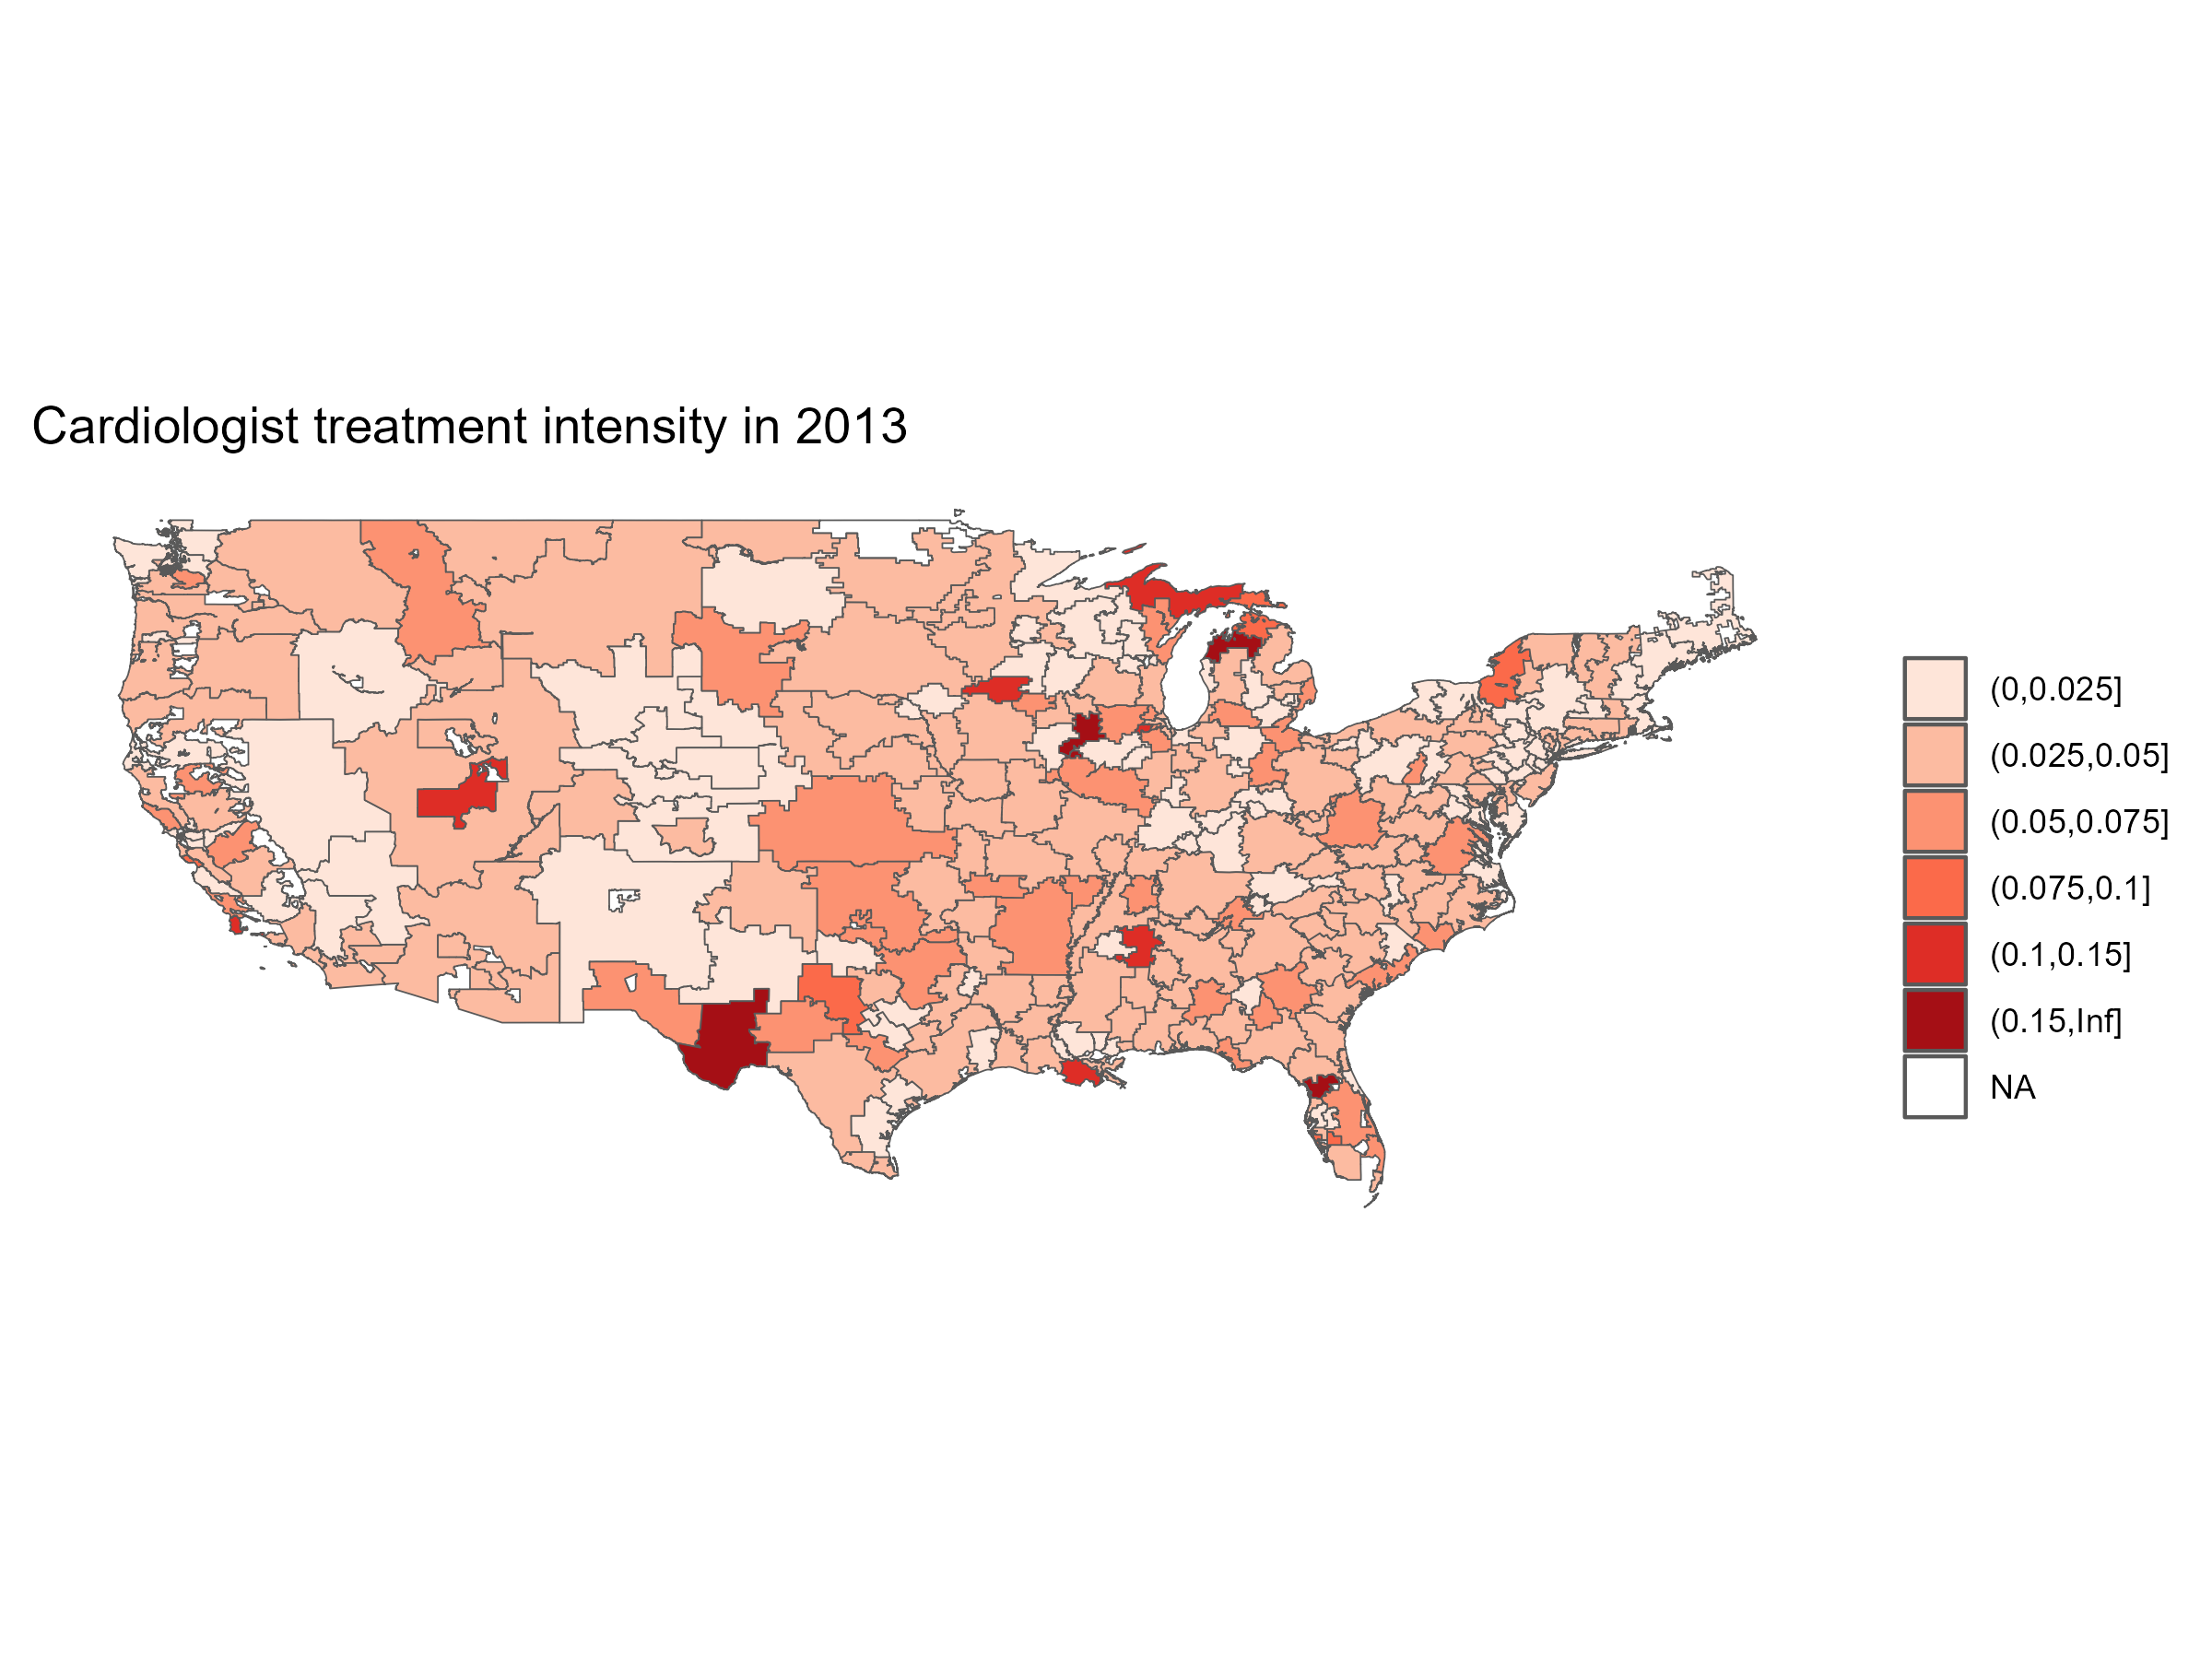
\includegraphics[width=\textwidth]{image/intensity/cardiointensebin2013.png}
    \end{figure}
    
\end{frame}

\begin{frame}{Next steps}
    \begin{itemize}
        \item Consider other measures of treatment style
            \begin{itemize}
                \item Re-evaluating definition of treatment intensity 
                \item ``Defensive" treatment style characterized by over-testing  
            \end{itemize}
        \vspace{2.5mm}
        \item Increase sample size
            \begin{itemize}
                \item Location data from Physician Compare
                \item Including additional specialties 
            \end{itemize}
    \end{itemize}
\end{frame}

\begin{frame}{Future work}
    \begin{itemize}
        \item Extend analysis to residency and fellowship 
            \begin{itemize}
                \item Currently webscraping training data for all doctors listed on Doximity 
                \item End goal: Determine the most important part of training pipeline
            \end{itemize}
        \vspace{2.5mm}
        \item Use this framework to study the effects of the medical training ``black box" 
            \begin{itemize}
                \item Technology adoption and diffusion 
                \item Research productivity
            \end{itemize}
    \end{itemize}    
\end{frame}

\begin{frame}[standout]
    \Large Thank you! 
    
    \vspace{5mm}
    \small shirley.cai@emory.edu
\end{frame}

\appendix

\begin{frame}{Treatment intensity measure} \label{intensity}
    \begin{itemize}
        \item Based on code description, I categorize all CPT codes billed to a cardiologist as treatment (invasive or non-invasive), diagnosis, office visit, or other. 
        \item All pathology and lab codes are assigned as diagnosis. 
        \item All patient-facing or patient-interaction codes are assigned office visit. 
        \item Ambiguous surgery codes (e.g., anesthesia), ambiguous infusions (e.g., saline IV), and non-cardiology related codes are assigned other. 
    \end{itemize}

    \hyperlink{rq}{\beamerbutton{Back}}
\end{frame}

\begin{frame}{Atlanta HRR} \label{atl-hrr}
    \begin{figure}
        \centering
        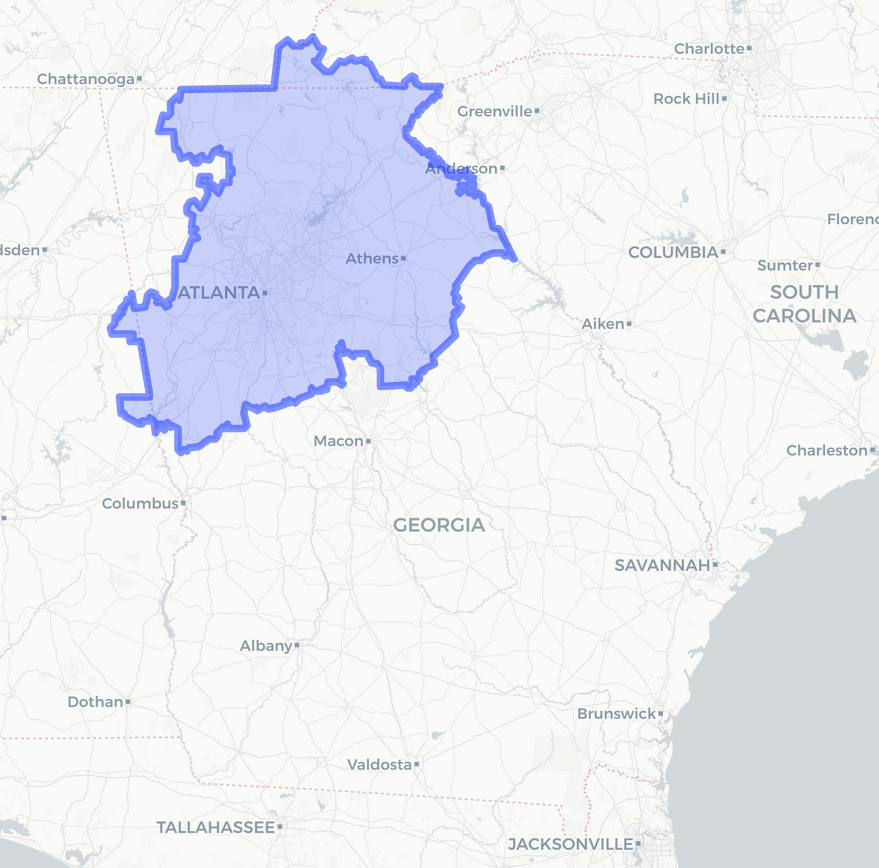
\includegraphics[width=0.45\linewidth]{image/atlanta-hrr.png}
    \end{figure}
    \hyperlink{data-ex}{\beamerbutton{Back}}
\end{frame}

\begin{frame}{Sample construction} \label{sample}
    A physician is included in the sample if 
        \begin{itemize}
            \item Their primary specialty is related to cardiology, including interventional cardiology, adult congenital heart disease, etc., but excluding cardiac surgeons
            \item Their graduated from an allopathic (MD) medical school in the US 
            \item Their current practice location is not missing 
        \end{itemize}

    \hyperlink{stats}{\beamerbutton{Back}}
\end{frame}

\nocite{*}

\begin{frame}[allowframebreaks]{References}
    \printbibliography[heading=none]
\end{frame}

\end{document}